\chapter{The switching model}
\label{chp:switching_model}

\graphicspath{{images/development_of_switching_model/}}

In this chapter I initially explore the effect of resolution on the Braginskii model, showing that a direct numerical implementation of~\ref{eq:brag_new} fails to capture the transition between isotropic and anisotropic viscosity in the vicinity of magnetic null points, when such an implementation is used in simulations performed at resolutions typical of modern 3d simulations. This motivates the implementation of a different model of viscosity: the switching model, which approximates the Braginskii tensor as an interpolation between the isotropic and parallel components. Three potential interpolation (or switching) functions are introduced: a phenomenological model derived from considering the probability of momentum transport in differing magnetic field strengths, and two functions based on coefficients of the Braginskii tensor. The development of the first model, referred to here as the von Mises switching function can be found in~\cite{mactaggartBraginskiiMagnetohydrodynamicsArbitrary2017}. Finally, I present the results of a suite of simulations performed at difference resolutions which illustrate the differences between the models and are used to gauge their efficacy.

\section{The transition from isotropic to anisotropic in the full Braginskii tensor}

In strong magnetic fields, the Braginskii tensor can be approximated by the purely parallel term while in weak or null fields, the tensor reduces to that of fully isotropic, Newtonian viscosity. Between these extremes the perpendicular and drift components of the tensor can become relevant~\cite{erdelyiResonantAbsorptionAlfven1995a}. Understanding how rapidly the Braginskii model transitions from isotropic to anisotropic with changing magnetic field strength is key to understanding the effect of resolution on the model.

\begin{figure}[t]
  \centering
  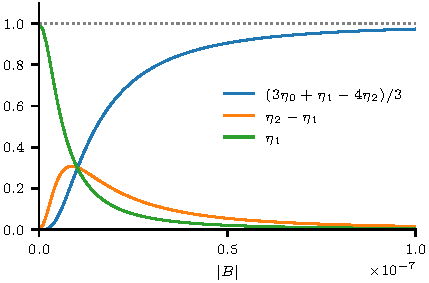
\includegraphics[width=0.5\linewidth]{brag_coeffs_2.pdf}
  \caption{Coefficients of the terms in equation~\ref{eq:brag_new2}, normalised against $\eta_0$.}%
  \label{fig:brag_coeffs2}
\end{figure}

The form of the Braginskii tensor as written in equation~\ref{eq:brag_new} is nearly in a form useful in understanding how quickly the tensor transitions from isotropic to anisotropic with changing magnetic field strength, since the isotropic component is completely isolated. Similarly, the parallel component can be isolated by further rewriting the tensor as,
\begin{eqnarray}\label{eq:brag_new2}
\ten{\sigma}_{\rm brag} = &&\frac{3\eta_0+\eta_1-4\eta_2}{3}\ten{W}^{(0)}\\% \label{new1} \\
\nonumber
& &+~ (\eta_2-\eta_1)[\ten{W}(\vec{b}\otimes\vec{b})+(\vec{b}\otimes\vec{b})\ten{W} - \frac{2}{3}(\ten{W}\vec{b}\cdot\vec{b})\ten{I}] \\%\label{new3}\\
\nonumber
& &+~ \eta_1\ten{W},%\label{new4}
\end{eqnarray}
Figure~\ref{fig:brag_coeffs2} presents the magnitudes of the coefficients of each of the terms in equation~\ref{eq:brag_new2}. Over the extremely small range between $|\vec{B}| = 0$ T and $10^{-7}$ T, the Braginskii tensor goes from completely isotropic to nearly completely parallel. Over the same range the coefficient corresponding to the perpendicular viscosity becomes relatively significant before tending to zero for large $|\vec{B}|$. The small transition region presents a problem in the numerical simulation of anisotropic viscosity, where the magnetic field strength likely changes more rapidly in space than can be captured by the coefficients in equation~\ref{eq:brag_new2}.

In the simulations of magnetic null points found later in section~\ref{sec:slow_null_point}, the magnetic field strength changes linearly in the $x$-direction. Given a typical grid spacing of $\Delta x = 0.01$, the jump in magnetic field from one grid point to the next is $5\times 10^{-5}$ T. This is much greater than the range over which the Braginskii tensor transitions between isotropic and anisotropic regimes and the viscous response is under-resolved as a result. For these simulations, the resolution would have to increase by a factor of $100$ to even begin to resolve the region of transition. Whether this region is physically significant or not is unknown, however, given the abundance of observable null points and their involvement in high-energy phenomena, it is possible that the isotropic (and perpendicular) viscosity near a null plays an important part in its dynamics. At the resolutions typically studied in general 3D MHD simulations (between $300$ and $1000$ grid points per dimension) the isotropic regions in the vicinity of null points are likely to be poorly resolved. This is particularly true in simulations where null points are not the main focus of the simulation, but are dynamically created by some process.

Computational solutions such as refining the mesh near the null or implementing a multigrid method may help to improve the resolution of a given simulation and better resolve the viscosity transition region, however approaches like these can be complex to implement in existing codes. An alternative to improving the resolution itself is to artificially scale $|\vec{B}|$ in the expression for the parallel Braginskii transport parameter~\ref{eq:perp_visc_coeff} in order to enlarge the isotropic region to resolvable scales. This is done by modifying the arguments of the parallel and perpendicular coefficients in~\ref{eq:perp_visc_coeff} and~\ref{eq:drift_visc_coeff}. Equations~\ref{eq:perp_visc_coeff} and~\ref{eq:drift_visc_coeff} are written in terms of the dimensionless parameter $x = \alpha |\vec{B}|$, where $\alpha$ is a physical parameter given by the expression $e \tau / m$. By artificially setting $\alpha$ to a value other than its physical value, the viscous response to changing $|\vec{B}|$ can be adapted to a given resolution.

Consider the effect of decreasing $\alpha$ on the coefficients shown in Figure~\ref{fig:brag_coeffs2}. Decreasing $\alpha$ exaggerates the size of the region near $|\vec{B}| = 0$ where the isotropic and perpendicular components are significant. In this way, $\alpha$ can be used as a controllable parameter to prescribe the size of the region of isotropic viscosity around a null point.

As well as exaggerating the region of isotropic viscosity, this approach requires exaggerating the region of perpendicular viscosity. To see this, consider the contributions to the field-aligned component of~\ref{eq:brag_new2} in a coordinate system where the field lies in the $z$-direction,
\begin{equation}
  \label{eq:z_aligned_field}
(\sigma_{brag})_{zz} = \frac{3\eta_0+\eta_1-4\eta_2}{3} W_{zz} + (\eta_2 - \eta_1) \frac{4}{3} W_{zz} + \eta_1 W_{zz} = \eta_0 W_{zz}.
\end{equation}
If the coefficient of the perpendicular component $\eta_2 - \eta_1$ are not scaled identically to the isotropic and parallel coefficients, the terms in~\ref{eq:z_aligned_field} no longer cancel appropriately and the field-aligned momentum transport is no longer independent of $|\vec{B}|$. Hence, scaling the coefficients in the Braginskii tensor to enlarge the isotropic region necessarily requires also scaling the size of the perpendicular region. While this may be a useful feature, creating a purely parallel-isotropic switching model offers an alternative while avoids the inclusion of perpendicular viscosity altogether.

\section{The switching model}

The switching model is a model of viscosity that approximates the full Braginskii tensor throughout most of the solar corona. By stripping out the perpendicular and drift components of the full Braginskii tensor, the switching model presents a cleaner, better-resolved model of viscosity. It focuses on what are, in many cases, the most physically important parts of anisotropic viscosity in the solar corona: the parallel and isotropic components. The idea at the core of the model is the interpolation between the parallel and isotropic tensors, mirroring the way in which the Braginskii tensor changes in strong and weak fields. For a general interpolation function $\tilde{s}(|\vec{B}|)$, henceforth referred to as a switching function, the switching model takes the form,
\begin{equation}
  \label{eq:switching_model_simple}
\ten{\sigma}_{\text{swi}} = \eta_0 \left( 1 - \tilde{s} \right) \ten{W} + \eta_0 \tilde{s} \ten{W}^{(0)},
\end{equation}
or
\begin{equation}
  \label{eq:switching_model}
\ten{\sigma}_{\text{swi}} = \eta_0 \left( 1 - \tilde{s} \right) \ten{W} + \eta_0 \tilde{s} \left[\frac{3}{2}(\ten{W}\vec{b}\cdot\vec{b}) \left( \vec{b} \otimes \vec{b} - \frac{1}{3}\ten{I} \right)\right].
\end{equation}
This trivially satisfies the requirement that the field-aligned component of momentum transport is independent of $|\vec{B}|$. The switching function may be thought of as a measure of the degree of anisotropy in the momentum transport, dependent on the local magnetic field strength, where $\tilde{s}(|\vec{B}|) = 0$ corresponds to totally isotropic and $\tilde{s}(|\vec{B}|) = 1$ corresponds to totally anisotropic.

\subsection{The von Mises switching function}

\begin{figure}[t]
  \centering
  \includegraphics[width=0.5\linewidth]{s_against_a.pdf}
  \caption{Plots of $s$, $s^2$ as functions of $a$ including the asymptotic limit as $a \to 0$.}%
  \label{fig:s_against_a}
\end{figure}

The von Mises switching function was originally developed by MacTaggart and Vergori\footnote{While I am cited as an author in the referenced paper, I became involved in the research after the switching model itself was developed. My contribution is in the numerical implementation of the model and the development and analysis of the simulations.}~\cite{mactaggartBraginskiiMagnetohydrodynamicsArbitrary2017}. In this model, a measure of anisotropy is developed by considering the direction of momentum transport to be governed by a particular orientation probability distribution, where a greater field strength increases the probability of the momentum transport aligning with the field. Choosing the von Mises distribution leads to the form
\begin{equation}
  \label{eq:switching_function}
s(|\vec{B}|) = \frac{3 \exp[2a]}{2\sqrt{2\pi a} \text{erfi}[\sqrt{2a}]} - \frac{1}{2}\left[ 1 + \frac{3}{4a} \right],
\end{equation}
where $a(|\vec{B}|)$ is a constitutive function which controls the sensitivity of the interpolation function to changes in magnetic field strength and erfi is the imaginary error function. The function and its squared is plotted in Figure~\ref{fig:s_against_a}. Where this model is used in throughout this thesis, the choice $a(|\vec{B}|) = a_0 |\vec{B}|^2$ is made, where $a_0$ is a parameter which effectively controls the size of the isotropic region near magnetic null points. 

\subsection{Braginskii-inspired switching functions}

Two alternatives to the phenomenological von Mises switching function~\ref{eq:switching_function} can be extracted from the Braginskii tensor itself. The tensor, written in the form~\ref{eq:brag_new2}, suggests two alternative interpolation functions, one based on the coefficient for the isotropic part $\eta_1$, and another based on the coefficient of the parallel part $(3\eta_0+\eta_1-4\eta_2)/3$. Figure~\ref{fig:brag_coeffs2} shows that the coefficient of the perpendicular term, $\eta_2 - \eta_1$ is not suitable as an interpolation function.

The Braginskii-inspired switching functions are easiest written using a form of $\eta_2(x)$ normalised against $\eta_0$,
\begin{equation}
  \label{eq:eta_function}
  \tilde{\eta}(x) = \eta_2(x)/\eta_0 = \frac{\tfrac{6}{5}x^2 + 2.23}{2.23 + 4.03 x^2 + x^4}.
\end{equation}
This allows us to define a new interpolation function based on the coefficient of the parallel part of the Braginskii tensor as
\begin{equation}
  \label{eq:alt_switching1}
s_{par}(x) = \frac{3+\tilde{\eta}(2x)-4\tilde{\eta}(x)}{3},
\end{equation}
and another based on the coefficient of the isotropic part,
\begin{equation}
  \label{eq:alt_switching2}
s_{iso}(x) = 1 - \tilde{\eta}(2x).
\end{equation}

\begin{figure}[t]
  \centering
  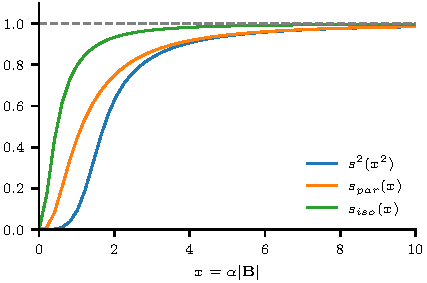
\includegraphics[width=0.5\linewidth]{alt_switching.pdf}
  \caption{The original switching function $s^2$ compared to the two possible interpolation function suggested by the Braginskii tensor. The interpolation rate of the functions are controlled by the parameters $a_0 = 36$ and $\alpha = 6$ which offer a direct comparison.}%
  \label{fig:alt_switching}
\end{figure}

Figure~\ref{fig:alt_switching} plots the two Braginskii interpolation functions and the switching function for parameter choices of $\alpha = 6$ and $a_0 = \alpha^2 = 36$. These parameter choices offer a direct comparison of the interpolation functions. The function $s_{par}$ shows the most similarity to the von Mises switching function, particularly the shallow slope near $|\vec{B}| = 0$, in contrast to the steeper slope of $s_{iso}$. 

\todo{little conclusion}

\subsection{Calibrating the interpolation functions}

The parameter $a_0$ controls the effective size of the isotropic region by controlling the degree to which the viscosity is anisotropic for a given field strength. At $a = 30$, $s \approx 0.95$ and the viscosity may be considered anisotropic. If the viscosity should be considered anisotropic around $|\vec{B}| = B_0$, $a_0 = 30/B_0^2$. This may be linked to the degree to which a magnetic null is resolved, as illustrated in the proceeding example. 

In the numerical experiments performed in chapter~\ref{chp:null_point_khi}, the magnetic field strength increases linearly with distance from the null point and the grid separation is found to be $\Delta x \approx 0.014$. If we wish to consider the isotropic region extending over a radius of, say, ten grid points, the field at $x = 10 \Delta x$ is $|\vec{B}| = 0.14$, resulting in a calibrated $a_0 \approx 1500$. 

\todo{add calibrating alpha too}


\section{Implementation of viscosity in Lare3D}

The two types of viscosity already present in the Lare3D code are shock and isotropic viscosities. Since shock viscosity is turned off for most numerical experiments presented in this thesis, I shall only detail the numerical implementation of isotropic viscosity, before discussing the implementations of the Braginskii and switching models.

\subsection{Review of the implementation of isotropic viscosity}

The isotropic viscous stress tensor is implemented in Lare3D as six 3D arrays, each storing the values for the six required components of a symmetric stress tensor. These are filled during the Lagrangian step using equation~\ref{eq:isotropic_viscous_tensor}, where the components of the strain rate tensor are calculated via equation~\ref{eq:rate_of_strain}. This stress tensor is used in the calculation of forces in the momentum equation and in the calculation of viscous heat contribution in the energy equation. This entire process is presented in detail below.

The strain rate tensor $\ten{W}$ is calculated in the code as \verb|s*|
\begin{verbatim}
sxx = (2.0_num * dvxdx - dvydy - dvzdz) * third
\end{verbatim}
for the diagonal elements \verb|sxx|, \verb|syy| and \verb|szz| and
\begin{verbatim}
sxy = dvxy * 0.5_num
\end{verbatim}
for the off-diagonal elements \verb|sxy|, \verb|sxz| and \verb|syz|. Since $\ten{W}$ is a symmetric tensor, only six components need to be calculated. The gradients of velocity, \verb|dv*|, are calculated using finite differences between appropriate velocity components, where the velocity is averaged over neighbouring grid points to ensure the resultant stress tensor is defined at the appropriate grid location. Note, the calculation of \verb|s*| in the code is a factor of a half smaller than the definition of $\ten{W}$ used in this thesis, equation~\ref{eq:rate_of_strain}. This is corrected for during the calculation of the viscous stress tensor, stored in the variable \verb|q*|, where a factor of two is included,
\begin{verbatim}
qxx(ix,iy,iz) = qxx(ix,iy,iz) + 2.0_num * sxx * rho(ix,iy,iz) * visc3
\end{verbatim}
and similarly for the other five components of the tensor. The multiplication by \verb|rho| at this point is cancelled out at a later stage.

The gradient of the tensor is used in the calculation of the forces in the momentum equation in the following way. The tensor values must be averaged to ensure the resultant gradient is correctly aligned with the velocity grid locations. Similar calculations are carried out for the other components of the stress tensor and force vector. This same code is used to include the anisotropic viscous stress tensors when they are enabled.
\begin{verbatim}
w1 = (qxx(ix ,iy ,iz ) + qxx(ix ,iyp,iz ) &
    + qxx(ix ,iy ,izp) + qxx(ix ,iyp,izp)) * 0.25_num
w2 = (qxx(ixp,iy ,iz ) + qxx(ixp,iyp,iz ) &
    + qxx(ixp,iy ,izp) + qxx(ixp,iyp,izp)) * 0.25_num
fx = fx + (w2 - w1) / dxc(ix)
\end{verbatim}

The viscous heat is calculated using
\begin{verbatim}
visc_heat(ix,iy,iz) = &
      qxy(ix,iy,iz) * dvxy  + qxz(ix,iy,iz) * dvxz &
    + qyz(ix,iy,iz) * dvyz  + qxx(ix,iy,iz) * dvxdx &
    + qyy(ix,iy,iz) * dvydy + qzz(ix,iy,iz) * dvzdz
\end{verbatim}
and, just as in the calculation of the forces above, this same code is used to calculate the viscous heat generated by the anisotropic viscous tensors when they are enabled.

\subsection{Implementation of the Braginskii tensor}

Since the contribution of a generic viscous stress tensor to the momentum and energy equations is already included in the numerical implementation of isotropic viscosity, the only new piece of code required to implement a new stress tensor is in the calculation of that stress tensor. The Braginskii tensor given by equation~\ref{eq:brag_new} is implemented in the following way and, when enabled, replaces the calculation of the isotropic viscous stress tensor. 

The four coefficients of the terms in equation~\ref{eq:brag_new} are calculated as
\begin{verbatim}
a = (3._num*visc3 + brag_visc1 - 4._num*brag_visc2)&
    / MAX(2._num*mB2**2, none_zero)
b = (brag_visc1 - visc3)/(2._num*mB2)
c = (brag_visc2 - brag_visc1)/(mB2)
d = brag_visc1
\end{verbatim}
where \verb|visc3| is the variable holding the value of $\eta_0$, \verb|brag_visc1| and \verb|brag_visc2| hold the values of $\eta_1$ and $\eta_2$, calculated via equation~\ref{eq:perp_visc_coeff}, and \verb|mB2| holds the value of $|\vec{B}|^2$. This calculation is performed in the following way
\begin{verbatim}
xi2 = (brag_alpha**2) * mB2
brag_visc_coeff = visc3*(6._num/5._num*xi2 + 2.23_num)&
                  / (2.23_num + 4.03_num*xi2 + xi2**2)
\end{verbatim}
where \verb|brag_alpha| is the physics-dependent $\alpha = e \tau / m$ TODO explain this earlier.

The quantity $(\ten{W} \vec{B}) \cdot \vec{B}$ and the tensor components of $\vec{B} \otimes \vec{B}$ are calculated using the following snippet.
\begin{verbatim}
calc_wbdotb = 2._num*(&
  (bx*sxx + by*sxy + bz*sxz)*bx &
+ (bx*sxy + by*syy + bz*syz)*by &
+ (bx*sxz + by*syz + bz*szz)*bz)

btxx = bx**2
btyy = by**2
btzz = bz**2
btxy = bx*by
btxz = bx*bz
btyz = by*bz
\end{verbatim}

This allows the Braginskii stress tensor to be calculated using
\begin{verbatim}
bsxx = wbdotb*(a*btxx + b) + 2._num*d*sxx &
  + 4._num*c*(btxx*sxx + btxy*sxy + btxz*sxz)
\end{verbatim}
and similar for the diagonal \verb|bsxx|, \verb|bsyy| and \verb|bszz| components. The off-diagonal components are calculated using the following snippet.
\begin{verbatim}
bsxy = wbdotb*a*btxy + 2._num*d*sxy &
  + 2._num*c*(btxx* sxy + btxy* syy + btxz* syz &
            +  sxx*btxy +  sxy*btyy +  sxz*btyz)
\end{verbatim}

Finally, the contribution from the Braginskii stress tensor is added to the total stress tensor using 
\begin{verbatim}
qxx = qxx + rho*bsxx
\end{verbatim}
and similar for the other components. A later calculation in Lare3D requires that the Braginskii stress tensor is multiplied by \verb|rho|.

\subsection{Implementation of the switching model}

The numerical implementation of the switching model is similar to the implementation of the Braginskii model detailed previously, with the exception of the tensor itself which is calculated using
\begin{verbatim}
bsxx = visc3*((1.0_num-s2)*sxx*2.0_num + 1.5_num*s2/MAX(mB2**2, none_zero)*wbdotb*(btxx - mB2*third))
\end{verbatim}
and similar for the diagonal \verb|bsxx|, \verb|bsyy| and \verb|bszz| components. The off-diagonal components are calculated using the following snippet.
\begin{verbatim}
bsxy = visc3*((1.0_num-s2)*sxy*2.0_num + 1.5_num*s2/MAX(mB2**2, none_zero)*wbdotb*(btxy))
\end{verbatim}

The numerical implementation of the interpolation function itself is discussed in the following section.

\subsection{Spline representation of the von Mises switching function}

For more efficient evaluation of~\ref{eq:switching_function}, it is approximated using a piecewise polynomial spline. For $a < 0.5051$, the function is clamped to $s=0$ and for $a > 29.41$, $s=1$. Between these cut-offs, $s^2$ is approximated using eight splines. The upper cut-off corresponds to the halo effect in the results presented later in section~\ref{sec:slow_null_point}.

\todo{add to this?}

\todo{plot the spline}

\section{Application to stressed null point}

\todo{reframe this chapter as a comparison of models}

\label{sec:slow_null_point}

As a test of the switching model in a non-trivial topology, a series of simulations of magnetic null points subjected to twisting motions were carried out. Newtonian (isotropic), full Braginskii and switching viscosities were used and the results compared.

\todo{describe ICs, BCs etc}

\subsection{Results}

\label{sec:slow_null_results}

The primary difference between isotropic and both anisotropic viscosity models is the magnitude and spatial distribution of the viscous heating. Isotropic viscosity overestimates the total heat generated by several orders of magnitude, when compared to either anisotropic model. The two anisotropic models differ in that the switching model vanishes where the Braginskii model does not, however it more clearly delineates the boundary between isotropic and anisotropic heating.

\subsubsection{Differences in viscous heating rates}

\begin{table}[t]
  \centering
  \caption{Total heat generated up to $t=10$ by each model of viscosity.}
  \label{tab:total_heating_slow_null}
  \begin{tabular}{ccccc}
Iso & Brag & Swi (von Mises) & Swi (par) & Swi (iso)\\
\midrule
$4.04 \times 10^{-3}$ & $5.25 \times 10^{-5}$ & $6.81 \times 10^{-5}$ & $7.80 \times 10^{-5}$ & $4.39 \times 10^{-5}$
\end{tabular}
\end{table}

Table~\ref{tab:total_heating_slow_null} shows the total heat generated by $t=10$ for each viscosity model. The isotropic model overestimates the viscous heating by approximately two orders of magnitude compared to any of the anisotropic models. The switching models all dissipate similar amounts of heat to the Braginskii model, indicating that these models are functioning correctly. The variance between each of the anisotropic models can be explained by considered how the isotropic and anisotropic parts of the tensors each contribute to the heating profile.

\begin{figure}[t]
    \centering
    \hfill
    \begin{subfigure}{0.32\textwidth}
      \includegraphics[width=1.0\linewidth]{iso_heating_iso_10.pdf}
      \caption{Isotropic}%
      \label{fig:iso_heating_iso_10}
    \end{subfigure}
    \hfill
    \begin{subfigure}{0.32\textwidth}
      \includegraphics[width=1.0\linewidth]{iso_heating_brag_10.pdf}
      \caption{Braginskii}%
      \label{fig:iso_heating_brag_10}
    \end{subfigure}
    \hfill
    \begin{subfigure}{0.32\textwidth}
      \includegraphics[width=1.0\linewidth]{iso_heating_switching_10.pdf}
      \caption{Switching (von Mises)}%
      \label{fig:iso_heating_switching_10}
    \end{subfigure}
    \begin{subfigure}{0.32\textwidth}
      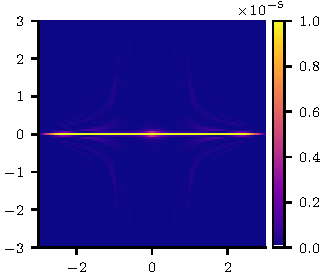
\includegraphics[width=1.0\linewidth]{iso_heating_switching2_10.pdf}
      \caption{Switching (par)}%
      \label{fig:iso_heating_switching2_10}
    \end{subfigure}
    \begin{subfigure}{0.32\textwidth}
      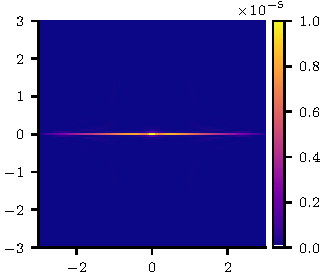
\includegraphics[width=1.0\linewidth]{iso_heating_switching3_10.pdf}
      \caption{Switching (iso)}%
      \label{fig:iso_heating_switching3_10}
    \end{subfigure}

    \caption{A comparison of the isotropic heating generated by the isotropic, full Braginskii and switching models at time $t=10$, sliced through $y=0$. Note the peak colour of the isotropic plot is an order of magnitude greater than that of the anisotropic models. The isotropic model overestimates local heating by an order of magnitude and heats more extensively throughout the null. The heating distribution generated by the isotropic switching model best matches that of the Braginskii model. Due to the numerical implementation of the von Mises switching function, some isotropic heating far from the null is neglected.}
\label{fig:isotropic_heating}%
\end{figure}

Figure~\ref{fig:isotropic_heating} shows the isotropic heating rate at time $t=10$ for each viscosity model. Isotropic viscosity heats at a generally greater rate than the anisotropic models, and the heating is distributed more extensively throughout the null. The boundary of the numerical cut-off, where isotropic viscosity turns off in the von Mises switching model, can be seen in figure~\ref{fig:iso_heating_switching_10}. The heating generated by the two Braginskii-inspired models show most similarity to that of the Braginskii model, with the isotropic-based switching model showing a nearly identical heating profile. This is to be expected since the coefficients of the isotropic contributions to the Braginskii and isotropic-based switching tensors are identical. The relative magnitude of the isotropic heating contributions for each anisotropic model reflects the total heat generated in table~\ref{tab:total_heating_slow_null}.

\begin{figure}[t]
    \hfill
    \begin{subfigure}{0.49\textwidth}
      \includegraphics[width=1.0\linewidth]{aniso_heating_brag_10.pdf}
      \caption{Braginskii}%
      \label{fig:aniso_heating_brag_10}
    \end{subfigure}
    \hfill
    \begin{subfigure}{0.49\textwidth}
      \includegraphics[width=1.0\linewidth]{aniso_heating_switching_10.pdf}
      \caption{Switching (von Mises)}%
      \label{fig:aniso_heating_switching_10}
    \end{subfigure}
    \hfill
    \begin{subfigure}{0.49\textwidth}
      \includegraphics[width=1.0\linewidth]{aniso_heating_switching2_10.pdf}
      \caption{Switching (par)}%
      \label{fig:aniso_heating_switching2_10}
    \end{subfigure}
    \hfill
    \begin{subfigure}{0.49\textwidth}
      \includegraphics[width=1.0\linewidth]{aniso_heating_switching3_10.pdf}
      \caption{Switching (iso)}%
      \label{fig:aniso_heating_switching3_10}
    \end{subfigure}
    \caption{A comparison of the anisotropic heating generated by the full Braginskii and switching models at time $t=10$. Close to the fan plane the Braginskii model shows notably greater anisotropic heating than any of the switching models. The switching models all appear similar though with minor differences near the null point.}
\label{fig:anisotropic_heating}%
\end{figure}

Figure~\ref{fig:anisotropic_heating} shows the contributions to viscous heating from the anisotropic parts of the Braginskii and switching tensors. The anisotropic heating generated by the Braginskii tensor is dominated by the perpendicular contribution near the fan plane. This reveals the potential issue with artificially increasing $\alpha$, that alongside increasing the size of the isotropic region, the extent of the perpendicular contributions are similarly enhanced. This may be a desirable feature of a model of anisotropic viscosity, however the switching models avoid this effect completely. In this way, the switching models provide a useful compromise.

\subsubsection{The effect of resolution on the size of the isotropic region}

\begin{table}[t]
  \centering
  \caption{Total heat generated up to $t=10$ by each model of viscosity for resolutions of $N=100$ and $500$.}
  \label{tab:slow_null_results_resolution}
  \begin{tabular}{c|cccc}
Model &  Brag & Swi (von Mises) & Swi (par) & Swi (iso)\\
\midrule
$N=100$ &  $5.74 \times 10^{-5}$ & $7.13 \times 10^{-5}$ & $8.39 \times 10^{-5}$ & $4.66 \times 10^{-5}$\\
$N=500$   & $5.25 \times 10^{-5}$ & $6.81 \times 10^{-5}$ & $7.80 \times 10^{-5}$ & $4.39 \times 10^{-5}$  \end{tabular}
\end{table}

\begin{figure}[t]
    \hfill
    \begin{subfigure}{0.49\textwidth}
      \centering
      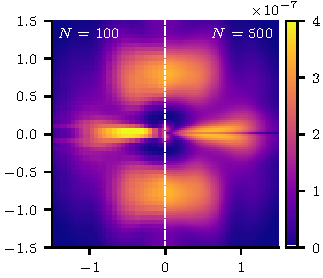
\includegraphics[width=1.0\linewidth]{diff_brag_resolution.pdf}
      \caption{Braginskii}%
      \label{fig:diff_brag_resolution}
    \end{subfigure}
    \hfill
    \begin{subfigure}{0.49\textwidth}
      \includegraphics[width=1.0\linewidth]{diff_switching_resolution.pdf}
      \caption{Switching (von Mises)}%
      \label{fig:diff_switching_resolution}
    \end{subfigure}
    \hfill
    \begin{subfigure}{0.49\textwidth}
      \includegraphics[width=1.0\linewidth]{diff_switching2_resolution.pdf}
      \caption{Switching (par)}%
      \label{fig:diff_switching2_resolution}
    \end{subfigure}
    \hfill
    \begin{subfigure}{0.49\textwidth}
      \includegraphics[width=1.0\linewidth]{diff_switching3_resolution.pdf}
      \caption{Switching (iso)}%
      \label{fig:diff_switching3_resolution}
    \end{subfigure}

    \caption{A comparison between the anisotropic heating rates produced by the Braginskii and switching models at resolutions of $100$ (left of each plot) and $500$ (right of each plot) grid points per dimension. Both plots are slices through $x=0$ at $t=5$. When the null point is less resolved (left half of both figures) Braginskii viscosity erroneously permits anisotropic heating at the null. At higher resolutions (left half of both figures) the null is better resolved and much less anisotropic viscous heating is found at the null. All switching models avoid this issue.}
\label{fig:anisotropy_bleeding}%
\end{figure}

\todo{Lower resolution further for low res runs}

\todo{what does it mean to say the models are accurate at low res??}

Identical simulations were run to those described in~\ref{sec:slow_null_results} but with the resolution reduced to $N=100$ per dimension. This allows a clear demonstration of the effect of poor resolution on the accurate estimate of anisotropic heating, even when $\alpha$ is artificially increased in the Braginskii model. While table~\ref{tab:slow_null_results_resolution} shows the global estimate of total viscous heat is relatively accurate at a low resolution, figure~\ref{fig:anisotropic_heating} shows that the spatial distribution of the heating rate is less so.

Figure~\ref{fig:anisotropy_bleeding} shows the heating rate produced by the anisotropic parts of the Braginskii and switching models and reveals the primary issue with the Braginskii model. When the resolution is too low to properly resolve the region around the null point, the Braginskii model erroneously heats anisotropically. This is primarily due to the artificially increased $\alpha$ enhancing the perpendicular components near the null point. This issue is mitigated by the switching models, all of which remove the perpendicular components of the Braginskii tensor. At the higher resolution of $N=500$ the von Mises switching model does remove a small portion of realistic anisotropic heating near the null. Both Braginskii-based switching models appear to approximate the Braginskii tensor more accurately. Away from the null the switching models give adequately similar results to the Braginskii model.

\section{Model efficiency}

In order to evaluate the real efficiency of each model of viscosity, a set of benchmark tests were run with the same physical setup as that of the test simulations found in section~\ref{sec:slow_null_point}, although changing the initial or boundary conditions should not affect the results. The resolution is set to $N=100$, all output is disabled, only one CPU core is used, and the simulations run for only $100$ timesteps. This number of timesteps allows the main loop of the simulation to run for a longer time than the overhead required to start and end the simulation, giving a more accurate estimate of the running time. The combination of the resolution and the number of timesteps results in the viscosity routines running $10^{8}$ times per simulation. The time is calculated via the linux \verb|time| command which reports millisecond accuracy. Due to other software running on the same machine, the total time can vary. To measure a more accurate running time, the test for each model is repeated $25$ times and the results averaged. The machine used to run these tests is a Dell all-in-one with a 4 core, Intel i7-6700 CPU running at 3.4 GHz and 16 GB of RAM. 

\todo{figure}

%Figure~\todo{fig} shows the average measured runtime for each model. Since the isotropic model requires only the calculation of the rate of strain tensor, it is the quickest. The Braginskii model, being the most complex, requires many additional calculations to be carried out and this is reflected in its relatively poor runtime. The switching models show similar efficiencies, worse than the isotropic model but significantly better than the Braginskii model, as expected from considering the number of required calculations. The differences between the runtimes of the different interpolation functions are slight, although the von Mises implementation appears moderately faster. 

\section{Conclusion}

This chapter details the development of the switching model, a new model of anisotropic viscosity specifically designed for use in numerical simulations of the solar corona. The model offers an alternative to the Braginskii model which captures the main physics while avoiding the problem of anisotropic heating at the null point itself. It does this by artificially enlarging the isotropic region surrounding magnetic null points. The switching model does this by exposing a tunable interpolation function which measures the degree of anisotropy (dependent on the local magnetic field strength) and interpolates between isotropic and fully field-aligned viscosity. Three candidate interpolation functions are presented and their accuracy, efficacy and computational efficiency compared. The switching model is found to be computationally more efficient than the Braginskii model and offers an acceptable approximation to it. 
